\documentclass[a4paper,12pt]{article}

\usepackage[english,russian]{babel}
\usepackage{indentfirst}
\usepackage[T2A]{fontenc}
\usepackage[utf8]{inputenc}
\usepackage[unicode=true]{hyperref}

\usepackage{amsmath,amssymb,amsfonts,longtable,hhline}
\usepackage{mathrsfs}
\usepackage{multimedia} 

\usepackage{geometry}
\geometry{left=2.5cm}
\geometry{right=1.5cm}
\geometry{top=2cm}
\geometry{bottom=2cm}

\usepackage{graphicx}
\usepackage{setspace}

\renewcommand{\baselinestretch}{1.5}
\makeindex

\begin{document}
  \large
  \begin{titlepage}
  \newpage
% \frenchspacing
\thispagestyle{empty} %нет нумерации 

{
  
  \begin{center}   
    Министерство образования и науки Российской Федерации\\ 
    \begin{spacing}{1.0} 
      федеральное государственное бюджетное образовательное учреждение \\ 
      высшего  образования \\ 
      «Иркутский государственный Университет» \\ 
      (ФГБОУ ВПО «ИГУ») 
    \end{spacing} 
    
    
    
    Институт математики, экономики и информатики 
    \\ 
    Кафедра методов оптимизации 
    
    
    
    ~\\[1.3cm] 
    
    { \bf 
      ВЫПУСКНАЯ КВАЛИФИКАЦИОННАЯ РАБОТА\\БАКАЛАВРА } 
    \\[0.3cm] 
    по направлению 01.03.02 Прикладная математика и информатика 
    \\ 
    профиль Математическое и компьютерное моделирование 
    \\[1.7cm] 
    
    { 
      Численная аппроксимация множества достижимости импульсной
      управляемой системы 
    } 
    
    
    ~\\[1.3cm] 
    
    \begin{multicols}{2} 
      \begin{flushleft} 
        \phantom{Четкая подпись} 
        \vspace{0.5cm} 
        
        \phantom{Четкая подпись} 
        \phantom{Четкая подпись} 
        \phantom{Четкая подпись} 
        \phantom{Четкая подпись} 
        \phantom{Четкая подпись} 
        \phantom{Четкая подпись} 
        \phantom{Четкая подпись} 
        \vspace{0.2cm} 
        
        \begin{spacing}{1.0} 
          Студента 4 курса очного отделения 
          \\группы 02422
          \\Апановича Данила Владимировича
          \vspace{0.5cm} 
          
          Руководитель: 
          \\д. ф.-м. н., профессор кафедры Методов оптимизации 
          \\ 
          \underline{\phantom{Четкая подпись}} Дыхта В.А. 
          \vspace{0.5cm} 
          
          Допущен к защите 
          \\Зав. кафедрой, д. ф.-м. н., профессор 
          \\ 
          \underline{\phantom{Четкая подпись}} Дыхта В.А. 
        \end{spacing} 
      \end{flushleft} 
    \end{multicols} 
    \vspace{1.3cm} 
    Иркутск~---~2016 г. 
  \end{center} 
}
\end{titlepage}

%%% Local Variables:
%%% mode: latex
%%% TeX-master: "rs-ids"
%%% End:

  \tableofcontents
  \pagebreak
  \chapter*{Введение}
\addcontentsline{toc}{chapter}{Введение}
\label{intro}

Существует ряд прикладных задач, связанных с динамическими
управляемыми системами, когда необходимо понять как будет вести себя
система при различных управлениях. Для этого необходимо понять, как
устроено множество достижимости системы, что даст наиболее полную
информацию о возможностях системы. Например оценка множества
достижимости позволяет понять, как ведет себя система при неизвестных
внешних воздействиях, скажем воздействие ветра на самолет во время 
посадки, и позволит определить --- не выходит ли его параметры за грань 
допустимых. Кроме того знание множества достижимости может помочь находить 
оптимальные управления для различных функционалов.

В управляемых системах возможны ситуации, когда за
очень короткий период времени происходит существенное изменение
некоторых параметров, описывающих функционирование системы.  Важные
примеры подобных ситуаций можно найти в математической экологии,
например, рациональное использование и охрана водных, земельных,
атмосферных, минеральных и энергетических ресурсов, аварийный разлив
нефти и моделирование распространения нефтяного пятна,  а также в
экономике, механике, ракетодинамике,  квантовой электронике (лазерное
излучение является импульсным по своей природе), робототехнике,
медиотерапии  и т.д. В частности, такие ситуации возникают при
моделировании реальных процессов, управление которыми осуществляется в
течение столь кратковременных промежутков, что их можно принимать как
мгновенные, а результаты воздействия приводят к быстрому изменению
процесса --- скачкам фазовой траектории моделируемой системы. Динамика
таких процессов в первом приближении может быть описана динамическими
системами  с разрывными траекториями и управлениями импульсного типа,
т.е. такими, при которых происходит резкое, скачкообразное изменение
состояния системы в отдельные моменты времени. 

Основная цель дипломной работы состояла в изучении возможности и
попытке реализовать алгоритм численного построения множества
достижимости импульсной управляемой системы билинейной
структуры. Наиболее важным реультатом стала реализация идеи
динамического программирования для алгоритма, что позволило в разы
увеличить скорость, с которой строится аппроксимация системы.


%%% Local Variables:
%%% mode: latex
%%% TeX-master: "rs-ids"
%%% End:

  \section{Постановка задачи. Необходимая теория}
\label{sec:theory}

% Расскажем об импульсных динамических системах подробнее и подведем %
% соотв. теоретическую базу.
%\section {Импульсные управления}
\subsection {Уравнение эйконала}
\label{sec:csdisttrack}

Предположим - у нас есть некоторая граница (замкнутая кривая в
двумерном пространстве), разделяющая область $\Omega$ на две подобласти:
внутреннюю и внешнюю. Предположим также, что кривая распространяется с
известной скоростью $F$, как показано на рисунке~\ref{fig:eikvis}. Для наших
потребностей достаточно предположить, что кривая расширяется, т.е. ее
движение направлено вовне текущей области $(F>0)$, а также
игнорируется касательная компонента движения, т.е. кривая
распространяется только по нормальному вектору, определенному $F$:

\begin{figure}[h]
  \centering
  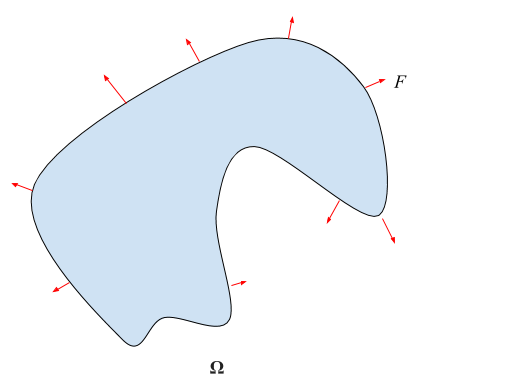
\includegraphics[width=0.5\linewidth]{img/eikonal_vision.png}
  \hfil \caption{распространение кривой со скоростью $F$}
  \label{fig:eikvis}

\end{figure}


Для того, чтобы определить положение кривой в каждой точке области. Мы
можем вычислить время прибытия $T$, когда впервые будет пересечена
каждая из точке $(x,y)$.

Если взять одномерный случай, то там мы можем вычислять расстояние как
произведение скорости на время, тогда мы можем записать уравнение для
функции $T$:

\begin{equation*}
  1 = F \frac{dT}{dx}
\end{equation*}

В пространствах более высокой размерности время прибытия T это решение
краевой задачи , также называемой уравнением эйконала.

\begin{equation}
  \label{eq:eikonal}
  \left\{ \begin{matrix}
      F(x) || \nabla T(x) || = 1, x \in \Omega \\
      T(x) = 0, x \in \Gamma
    \end{matrix}\right.
\end{equation}

Здесь $\Omega$ -- это область в $\mathbb{R}^n$, $\Gamma$ -- начальная
позиция кривой, $\nabla$ обозначает градиент, и $\|| \cdot ||$ является
Евклидовой нормой.

Стоит отметить, что эволюция кривой и время первого прибытия
отличаются. Для иллюстрации рассмотрим распространение кривой со
скоростью $F \equiv 1$, как представлено на Рисунке~\ref{fig:prpgt-eik}

\begin{figure}[h]
  \centering
  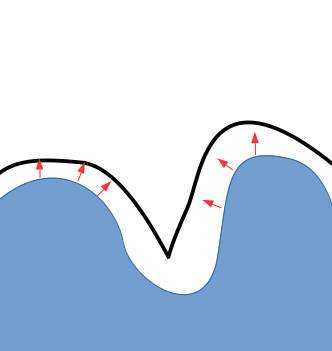
\includegraphics[width=0.3\linewidth]{img/propagate_eikonal.png}
  \hfil \caption{распространение кривой со скоростью $F = 1$}
  \label{fig:prpgt-eik}

\end{figure}

Жирная линия указывает где будет кривая на следующем шаге.  Предположим
теперь мы хотим заглянуть дальше, тогда мы получим следующую картину
на рисунке~\ref{fig:swallow-ex} кривая пройдет сквозь себя, соорудив
так называемый \textit{ласточкин хвост}. Чем он плох? Мы в некоторых
точках получаем многозначную функцию, чего нужно избегать. В
\cite{S1999}, Сетиан описывает эту ситуацию, как если мы рассмотрим
фронт распространения кривой, как фронт распространения огня, тогда
то, что было однажды сожжено, второй раз не сжигается.  Следовательно
нам стоит выбрать в каком-то смысле физически корректное решение с
фигурой, как на рисунке~\ref{fig:correct-exmp}

\begin{figure}[h]
  \centering
  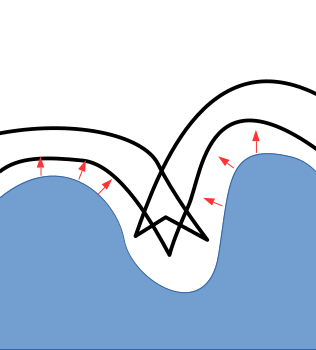
\includegraphics[width=0.3\linewidth]{img/swallow-tail-example.png}
  \hfil \caption{Пример ласточкиного хвоста}
  \label{fig:swallow-ex}

\end{figure}

\begin{figure}[h]
  \centering
  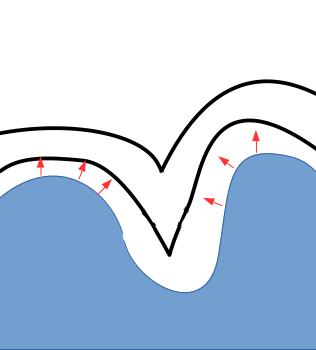
\includegraphics[width=0.3\linewidth]{img/corrct-example.png}
  \hfil \caption{Пример корректного решения}
  \label{fig:correct-exmp}

\end{figure}

Уравнение~\eqref{eq:eikonal} является частным случаем \textit{уравнения
Гамильтона-Якоби} первого порядка, которое в статичном случае выглядит
следующим образом:

\begin{equation}
  \label{eq:hje}
  \left\{ \begin{matrix}
      H(x, Du) = 0,\text{на } \mathbb{R}^n \times (0,\infty) \\
      T(x) = 0,  \text{на } \mathbb{R}^n \times \{t = 0\},
    \end{matrix}\right.
\end{equation}
где Гамильтониан $H = H(x,Du)$ непрерывная вещественная функция на
$\mathbb{R}^n \times \mathbb{R}^n$ и $\phi : \mathbb{R}^n \rightarrow
\mathbb{R}$ -- начальная функция.

В общем случае это уравнение не имеет классических $C^1$
решений. Проблема эта имеет решение в обобщенных решениях, которые
непрерывны и удовлетворяют данному уравнению в частных производных
почти всюду.

%%% Local Variables:
%%% mode: latex
%%% TeX-master: "eikonal_solver"
%%% End:

  \chapter{Алгоритмы аппроксимации}
\label{ch:algrhtms}


В этой главе опишем два подхода для численной аппроксимации множества
достижимости. Первый подход, основывался на идее полного перебора всех
возможных управлений, что не позволяло хоть какое-то его адекватное
практическое применение для решения задач.  Второй подход, основанный
на численном решении волнового уравнения Эйконала и его связи с
уравнением Гамильтона-Якоби, позволил использование быстрых алгоритмов
поиска кратчайшего пути на сетке. Появился в результате серьезного
переосмысления первого.

\section{Переборный алгоритм}
\label{sec:simple_alg}

Отметим, что интегральное ограничение в
\eqref{system_s} и условия, накладываемые на функции $f(t,x)$ и $G(t,x),$
обеспечивают компактность и связность множества достижимости, а
также его непрерывную зависимость от величины интегрального
ресурса управления $V$. Проведем преобразование системы
\eqref{system_s} при помощи разрывной замены времени. 

Аппроксимация множества достижимости импульсной системы осуществляется по
следующей схеме:
\begin{enumerate}
\item Задается разбиение отрезка $[b-a,b-a+V]$ на $k$ частей точками:
  $ \Delta=\big\{ \tau_{0}, \tau_{1}, \ldots, \tau_{k} \big\}, $ где
  $\tau_{0}=b-a< \tau_{1}< \ldots < \tau_{k}=b-a+V$. Положим
  $h_i:=\tau_{i}-\tau_{i-1},$ $i=\overline{1,k}$;
\item для каждого фиксированного $\tau_{i},$ $i=\overline{1,k},$
  численно строится оценка множества достижимости вспомогательной
  системы $\mbox{\bf R}_i ,$ т.е.
  ${\mathcal R}_{\mbox{\rm auxiliary}}(\tau_{i}) \approx \mbox{\bf
    R}_i$;
\item оценку множетсва достижимости исходной импульсной системы \eqref{system_s} с
  разрывными траекториями получаем путем объединения множеств
  $\mbox{\bf R}_i$, $i=\overline{0,k},$ т.е.
  $ {\mathcal R}_M(b)\approx \bigcup_{i=0}^k \mbox{\bf R}_i$.
\end{enumerate}


Рассмотрим кусочно-постоянные управления
$(\omega_0(\cdot),\omega_1(\cdot),\omega_2(\cdot))$, соответствующие
$\Delta$ и удовлетворяющие условиям:
\begin{equation*}
  \begin{array}{l}
    \sum_{j=1}^k \omega_{0j}h_j=b-a\\
    \omega_{0j}, \omega_{1j}, \omega_{2j} \geq 0,\\ 
    \omega_{0j}+ \omega_{1j}+ \omega_{2j} =1, \ \ j=\overline{1,k}.
  \end{array}
\end{equation*}

Пусть $\Omega(\Delta)$ --- множество всех таких управлений, компоненты
которых принимают значения либо 0 либо 1. Тогда всевозможные выпуклые
комбинации элементов $\Omega$ дают все кусочно постоянные управления,
соответствующие выбранному разбиению.  Заметим, что количество
элементов в $\Omega(\Delta)$ не превышает $m^{k-q} C_k^q$, где
$q=\left[\frac{b-a}{h}\right]$ --- число отрезков, на которых
$\omega_{0j}=1$.  Элементы $\Omega(\Delta)$ полностью определяются
номерами компонент с единичными значениями. Например, если $T=[0,1]$,
$\tau_1=3$ --- конечный момент времени во вспомогательной системе,
$k=3$ --- количество подотрезков разбиения, то $\Omega(\Delta)$
задается множеством
$\left\{122; 123 ; 132 ; 133 ;212 ; 213; 312 ; 313 ; 221; 231 ; 321 ;
  331 \right\}$.
Затем мы строим точки множества достижимости для каждого управления из
$\Omega(\Delta)$, и, если нужно, их попарные выпуклые комбинации.

Алгоритм такого имеет очень серьезный недостаток --- экспоненциальную
вычсилительную сложность, как это показано выше в оценук мощности
множества $\Omega(\Delta)$. Данный недостаток, накладывает серьезные
ограничения на практическую применимость данного алгоритма.

\section{Волновой алгоритм}
\label{sec:wave_alg}
Введем равномерную сетку на области измененияи на отрезке времени и
разделим два способа изменения состояния системы — дрейф системы и
движение под воздействием импульса.  Для всех узлов можно посчитать
стоймость перехода из него в соседние, получая при этом взвешенный
граф, для импульсного воздействия.

Стартовому узлу присваиваем максимальный ресурс системы \eqref{system_s}. Затем
подсчитываем значение ресурса для соседних узлов, после этого соседние
для них и т.д пока не значение ресурса в узлах не станет нулевым. При
этом, если в один и тот же узел приходят разные значения ресурса,
записывается большее — таким образом мы найдем насколько далеко можно
добраться из стартовой точки, т.е. границу МД системы. \eqref{system_s}. Таким
образом реализуется идея поиска кратчайшего пути на графе в смысле
оптимального расходования ресурса управления системы.

Далее мы действуем дрейфом на все полученные точки, в течении одного
малого шага отрезка , смещая тем самым узлы. После чего попытаемся из
кадого узла подействовать импульсом (если это позволяет попасть в
соседний узел с большим значением .  Таким образом действуя по
переменке дрейфом и импульсным скачком мы пройдем весь отрезок времени
и получим точки МД для системы.

  \section{Примеры}
\label{sec:samples}

\subsection{Евклидово расстояние}
\label{sec:simple-eikonal}

Рассмотрим несколько примеров и приложений для алгоритмов, описанных
выше. Для начала разберем простой пример:


\begin{equation}
  \label{eq:eik-sur}
  \begin{cases} \begin{array}{ll}
      \| \nabla T(x) \| = 1, x \in \Omega \\
      T(x) = 0, x \in \Gamma
    \end{array}\end{cases}
\end{equation}

В простейшем случае, мы считаем, что функция $F$ уравнение
\eqref{eq:eikonal} является константой и равна единице, т.е. после
дискретизации в каждой точке $\Omega$ функция $F$ принимает значение
$1$. Тогда решением будет концентрические окружности
рисунок~\ref{fig:eikonal-surface}, если же его рисовать в трехмерном
пространстве (см. Рисунок~\ref{fig:eikonal-surface-3d}).

\begin{figure}[H]
  \centering
  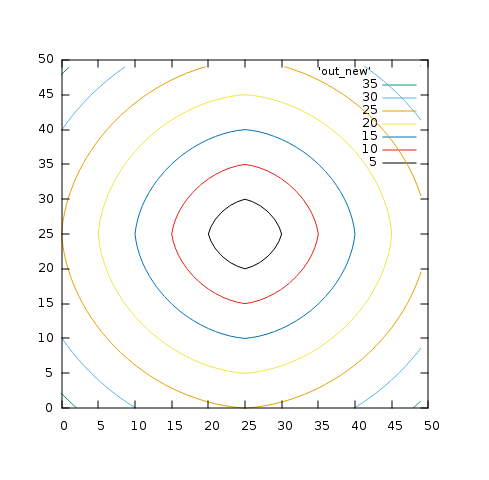
\includegraphics[width=0.7\linewidth]{img/eikonal_simple_surface.png}
  \hfil \caption{Линии уровня эйконала с $F\equiv 1$ }
  \label{fig:eikonal-surface}
\end{figure}

\begin{figure}[H]
  \centering
  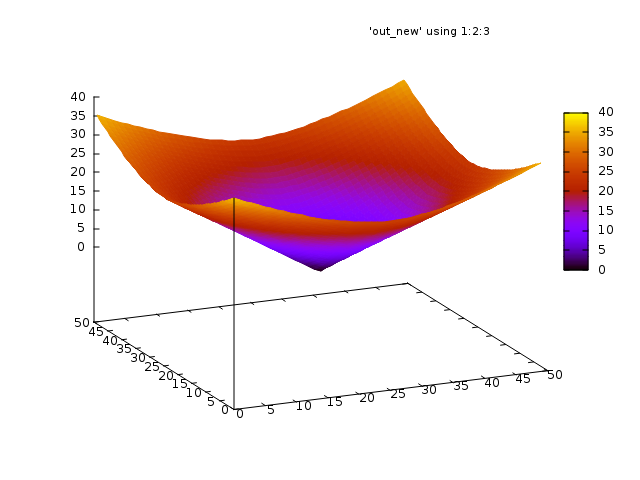
\includegraphics[width=\linewidth]{img/eikonal_simple_3d.png}
  \hfil \caption{Трехмерный график численного решения эйконала с
    $F\equiv 1$}
  \label{fig:eikonal-surface-3d}
\end{figure}

Если мы добавим барьер для распространения волн, т.е. в точках лежащих
на некотором прямоугольнике установим значение $0$. Мы получим
следующий результат. Смотри рисунок~\ref{fig:barier_surface}.

\begin{figure}[H]
  \centering
  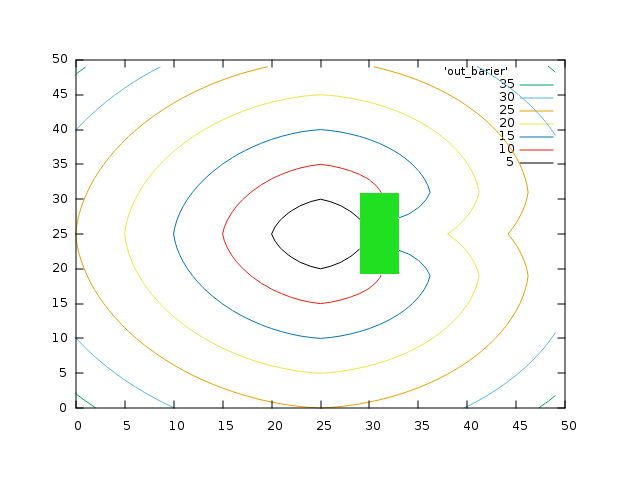
\includegraphics[width=\linewidth]{img/barier_surface.png}
  \hfil \caption{Линии уровня эйконала с $F\equiv 1$, с препятствием}
  \label{fig:barier_surface}
\end{figure}

\subsection{Множество достижимости импульсной системы}
\label{sec:ids}

В работах \cite{AVS2016, AV2015_1,AV2015_2} предлагалось считать
множество достижимости импульсной управляемой системы \cite{D2003}. В
использованном в тех работах методе, были существенные ограничения на
систему ограничений на управление. Для описаний ограничений на
управлении использовалась $l_1$ метрика. Методы численных решений
уравнений эйконала позволяют нам использовать евклидову метрику,
правда за счет некоторого упрощения управляемых систем.

Для начала взглянем на обычную управляемую систему, расширение
множества траекторий которой и приводит к импульсной системе. Будем
работать с системой следующего вида. 

\begin{equation}
  \label{system_s}
  \begin{array}{l}
    \dot{x}(t)=E \cdot F(x)v(t), \quad x(0)=x_0, \\[8pt]
    v(t)\geq 0  \qquad \forall\, t\in T = [0,t_1], \qquad
    \displaystyle\int_{0}^{t_1} ||v(t)||dt\leq V.
  \end{array} 
\end{equation}

Здесь
\begin{itemize}
  \item $E$ --- единичная матрица.
  \item $||v||:=\sqrt{v_1^2+v_2^2}$
  \item $x(\cdot)$ --- абсолютно непрерывная вектор-функция
    (траектория), $x(t)\in {\mathbb R}^n,$
  \item $v(\cdot)$ --- измеримая существенно ограниченная
    вектор-функция (управление),
  
  \item $V$ --- заданная величина интегрального ресурса управления
    $v$.
\end{itemize}

Пару функций $\bigl(x(\cdot),v(\cdot)\bigr),$ удовлетворяющих
системе \eqref{system_s}, будем называть процессом системы \eqref{system_s}.

Будем предполагать, что вектор-функция $f$ является функцией из
$L_{\infty}(T,\mathbb{R}^2)$.
     
Множество обычных траекторий системы \eqref{system_s} будет состоять
из функций, имеющих равномерно ограниченные полные вариации на отрезке
$T$. Следовательно, любая последовательность траекторий будет
содержать подпоследовательность, поточечно сходящуюся к некоторой
функции ограниченной вариации. Именно такие функции, являющиеся
поточечными пределами последовательностей обычных траекторий, в
дальнейшем будут называться разрывными (или обобщенными) решениями
системы \eqref{system_s}.

 Рассмотрим систему \eqref{system_d} соответствующую системе
\eqref{system_s}.

\begin{equation}
  \label{system_d}
  \begin{array}{l}
    dx(t)=f\big(t,x(t)\big)dt+G\big(t,x(t)\big)\pi(\mu), \quad
    x(0)=x_0, \\[8pt]
    \pi(\mu) \in \mathcal{W}(T)
  \end{array} 
\end{equation}

Здесь $T=[0,t_1]$ --- заданный отрезок времени, $x(\cdot)$ ---
непрерывная справа на $(0,t_1]$ функция ограниченной вариации, $x(t)
\in \mathbb{R}^2$. Решения системы \eqref{system_d}, соответсвующие
управлению $\pi(\mu)$, понимаются как решения интегрального уравнения
с мерой
\begin{equation*}
  x(t) = x_0  + \int_0^t E\cdot F(t,x(t)) \mu_c(dt) +
  \sum_{s \le t,\\s \in S_d(\mu)} (z_s(d_s) - x(s-)), \quad t \in (0,t_1]
\end{equation*}
где для каждого $s \in S_d(\mu)$ функция $z_s(\cdot)$ --- решение
дифференциального уравнения
\begin{equation*}
  \frac{dz_s(\tau)}{d\tau} = E\cdot f(s,z_s(\tau))\omega_s(\tau), \quad z_s(0)=x(s-)
\end{equation*}

Таким образом, при расширении системы \eqref{system_s} и переходе к
соответствующей импульсной системе \eqref{system_d} мы к обычным
(абсолютно непрерывным) траекториям добавляем все частичные
поточечные пределы последовательностей обычных
траекторий. Полученное множество будем называть множеством
траекторий импульсной системы, соответствующей \eqref{system_s} и будем
обозначать импульсную систему символом \eqref{system_d} Поясним,
что если в системе \eqref{system_d} траектории могут иметь скачки,
то их обобщенные производные будут содержать дельтообразные
составляющие --- импульсы; следовательно, импульсы появятся в
соответствующих управлениях, отсюда и названия импульсной системы и
импульсного управления.


Функция ограниченной вариации $x(\cdot)$ называется траекторией
импульсной системы \eqref{system_d} (или обобщенным (разрывным)
решением системы \eqref{system_s}), если найдется такая последовательность
траекторий системы \eqref{system_s} $\bigl\{x_k(\cdot)\bigr\}$, что выполняется
условие 
\begin{equation*}
  x_k(t)\to x(t) \quad  \forall \, t\in [0,T].
\end{equation*}

Определим \emph{множество достижимости} в момент  времени $t=t_1$
импульсной системы \eqref{system_d}. Обозначим это множество через 
$ {\mathcal R}_V(t_1)$. Это множество из  пространства ${\mathbb R}^n$
(конечномерное  множество), оно состоит из точек $x_b,$ в  которые в
момент $t=t_1$ попадают траектории  системы \eqref{system_d}, выходящие
в начальный  момент из начальной точки $x_0$.

Возьмем пример динамической системы:

\begin{equation*}
  \begin{aligned}[b]
    &\dot{x_1}(t) = (1/((x_1(t)+0.1) * (x_2(t)+0.1))v_1(t), & x_1(0)=50\\
    &\dot{x_2}(t) = (1/((x_1(t)+0.1) * (x_2(t)+0.1))v_2(t), & x_2(0) = 50\\[8pt]
    &v_1(t) \ge 0, v_2(t) \ge 0 \\
    &\int_{0}^{1} \sqrt{(v_1(t)^2) + (v_2(t))^2} dt \le V
  \end{aligned}
\end{equation*}

Множеством достижимости для конкретного $V$ здесь будут все значения
решения, которые меньше или равны заданному $V$. Численные методы
решения эйконала порождают интегральную воронку: все возможные
множества достижимости для значения $V \in [0,V_{max}]$

На рисунке~\ref{fig:impulse-example-levels} представлено такая
интегральная воронка через линии уровня.

\begin{figure}[H]
  \centering
  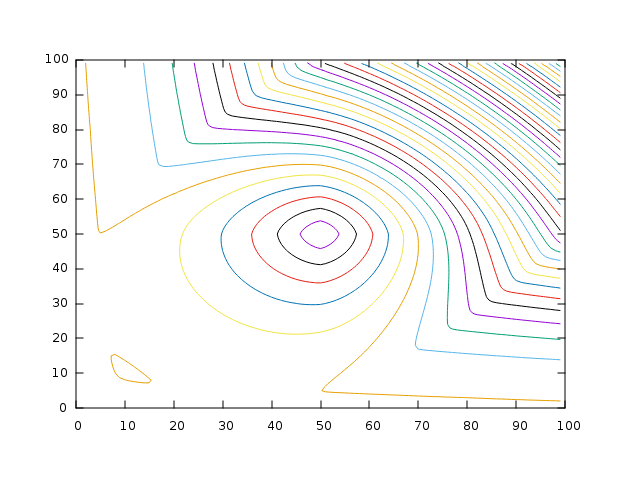
\includegraphics[width=0.5\linewidth]{img/impulse-example-levels.png}
  \hfil \caption{Линии уровня множества достижимости}
  \label{fig:impulse-example-levels}
\end{figure}

В виде трехмерной поверхности график можно увидеть на
рисунке~\ref{fig:impulse-example}

\begin{figure}[H]
  \centering
  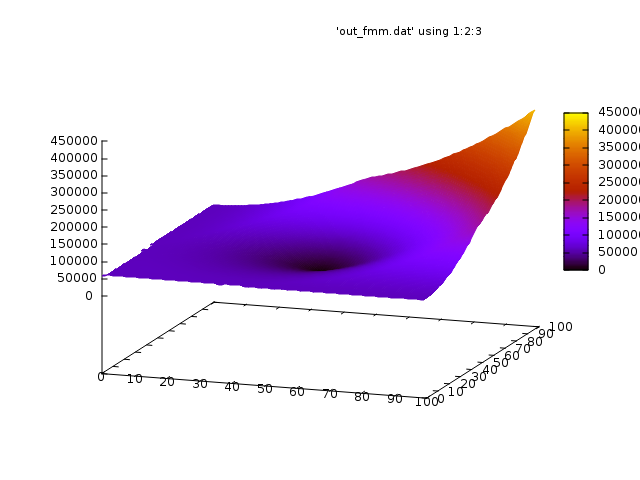
\includegraphics[width=\linewidth]{img/impulse-example.png}
  \hfil \caption{Интегральная воронка в трехмерном виде}
  \label{fig:impulse-example}
\end{figure}


\subsection{Shape from shading}
\label{sec:shape-from-shading}

Еще одним важным приложением численных алгоритмов решения уравнения
эйконала является задача восстановления по черно-белой картинке (или
фотографии) форму исходного объекта \cite{SFS2009,JDM2008}. Это понятие также
не переводится в русскоязычных публикациях.  Дословно это понятие
значит построение поверхности от тени. На изображении, лишенном цвета,
нашему глазу предоставляется информация о яркости соответствующей
точки. Наш глаз может благодаря ей строить форму объекта.  

Яркость изображения пропорциональна излучению от поверхности к
наблюдателю

\begin{equation}
  \label{eq:sfs:1}
  E_i=\mu L_s,
\end{equation}

где параметр $\mu$ зависит от параметров камеры (таких как диаметр
линзы, фокальное расстояние и т.д.).
Мы полагаем, что источник освещения один и находится примерно там же,
где и глаз наблюдателя. Кроме того отсутствуют отражения. Яркость
изображения пропорциональна излучению поверхности, изображенной на
нем. В этом случае отношение между излучением точки поверхности с
нормалью в этой точке и направлением к источнику света описывается 
Двулучевой функцией отражательной способности (ДФОС), которая является
константой для Ламбертиановской поверхности.

\begin{equation}
  \label{eq:sfs:4}
  L_s=\frac{\alpha}{\pi}E_s,
\end{equation}
где $\alpha$ --- альбедо, а $E_s$ --- интенсивностью
излучения. Наконец, интенсивность излучения $E_s$ определяется как:

\begin{equation}
  \label{eq:sfs:5}
  E_s = I_0\frac{cos(\theta_i)}{r^2},
\end{equation}
где $I_0$ это интенсивность источника света, $r$ --- расстояние между
источником света и точкой поверхности и $theta_i$ --- угол между
нормалью к точке поверхности и направлением на источник света.

Из \eqref{eq:sfs:1}, \eqref{eq:sfs:4} и \eqref{eq:sfs:5} получим яркость
изображения:

\begin{equation}
  \label{eq:sfs:6}
  E_i = \sigma\frac{cos(\theta_i)}{r^2},
\end{equation}
где $\sigma$ это постоянный коэффициент, связанный с параметрами
системы формирования изображения, интенсивности источника света и
альбедо поверхности.

Мы можем получит формулы для того, чтобы преобразовать яркость в
коэффициент, пропорциональный углу наклона нашей поверхности.  На
языке python был написан скрипт (листинг 8), который переводит
информацию по яркости изображения в такой параметр, т.е. чем выше
яркость, тем меньше в этой точке наклон поверхности относительно
ортогонального к нам. Тем самым мы получаем $F$ для уравнения
эйконала, по которой ищем решение. Оно и будет той самой поверхностью,
которую нам нужно достать из фотографии

\vspace{1em} Листинг 8 --- Скрипт преобразования изображение в $F$ для
уравнения эйконала \normalsize
\begin{verbatim}
#!/usr/bin/env python

from PIL import Image
import scipy as sc
import sys
import math

def main():
    im = Image.open(sys.argv[1])
    print im.height* im.width, 3
    data = sc.asarray(im.convert("L"))

    out = sc.empty([im.height, im.width])

    max_out = 0
    
    max_val = data.max()
    lst = []
    for i in range(len(data)):
        for j in range(len(data[i])):
            if abs(data[i][j]) > 0.01:
                tst = math.sqrt(
          (1.0*max_val/data[i][j])**2 - 1)
                if abs(tst) > 0.1:
                    out[i][j] = 1.0/tst
                else:
                    out[i][j]= sc.inf
            else:
                out[i][j]= 0
            if out[i][j]>max_out:
                max_out = out[i][j]

    for i in range(len(data)):
        for j in range(len(data[i])):
            if data[i][j]==max_val:
                print i,j,out[i][j],0
            else:
                print i,j,out[i][j],sc.inf

if __name__ == '__main__':
    main()
\end{verbatim}
\large

Далее приведем несколько примеров картинок и трехмерных поверхностей,
полученных на них. Сперва было построено тестовое синтетическое
изображение сферы для тестирования алгоритма: рисунки~\ref{fig:ex:1:in} 
и ~\ref{fig:ex:1:out}

\begin{figure}[H]
  \centering
  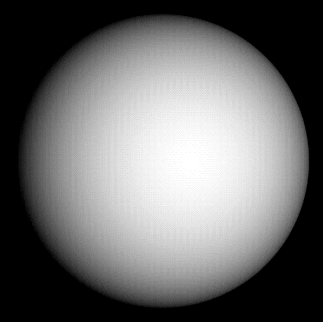
\includegraphics[width=0.5\linewidth]{img/sphere_in.png}
  \hfil \caption{Сфера исходное изображение}
  \label{fig:ex:1:in}
\end{figure}

\begin{figure}[H]
  \centering
  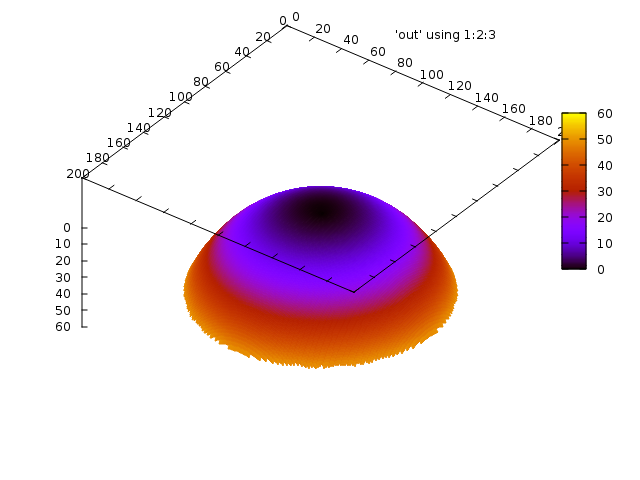
\includegraphics[width=0.5\linewidth]{img/sphere.png}
  \hfil \caption{Трехмерная поверхность сферы по фотографии}
  \label{fig:ex:1:out}
\end{figure}

Затем было решено попробовать несколько стандартных фигур, в работах
по компьютерному зрению и 3D моделированию: чайник
(рисунки~\ref{fig:ex:2:in} и ~\ref{fig:ex:2:out}) и маска Моцарта
(рисунки~\ref{fig:ex:3:in} и ~\ref{fig:ex:3:out}).

\begin{figure}[H]
  \centering
  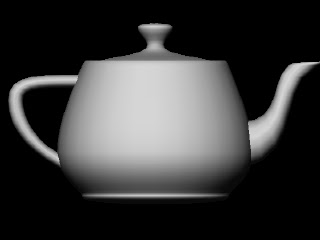
\includegraphics[width=0.5\linewidth]{img/teapot_in.jpg}
  \hfil \caption{Чайник исходное изображение}
  \label{fig:ex:2:in}
\end{figure}

\begin{figure}[H]
  \centering
  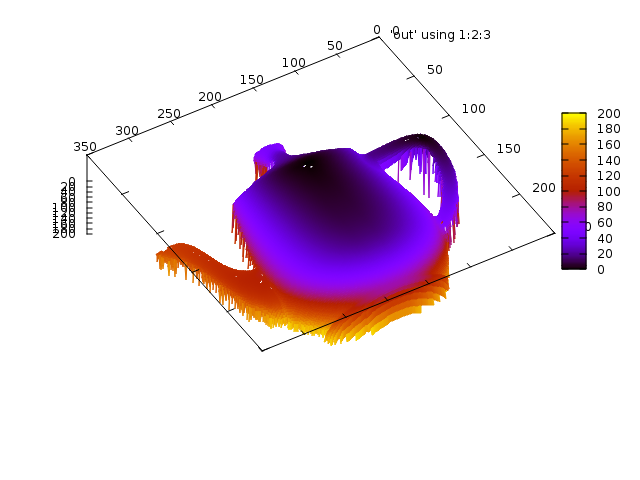
\includegraphics[width=0.5\linewidth]{img/teapot.png}
  \hfil \caption{Трехмерная поверхность чайника по фотографии}
  \label{fig:ex:2:out}
\end{figure}

\begin{figure}[H]
  \centering
  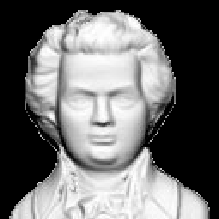
\includegraphics[width=0.5\linewidth]{img/mozart_in.png}
  \hfil \caption{Моцарт исходное изображение}
  \label{fig:ex:3:in}
\end{figure}

\begin{figure}[H]
  \centering
  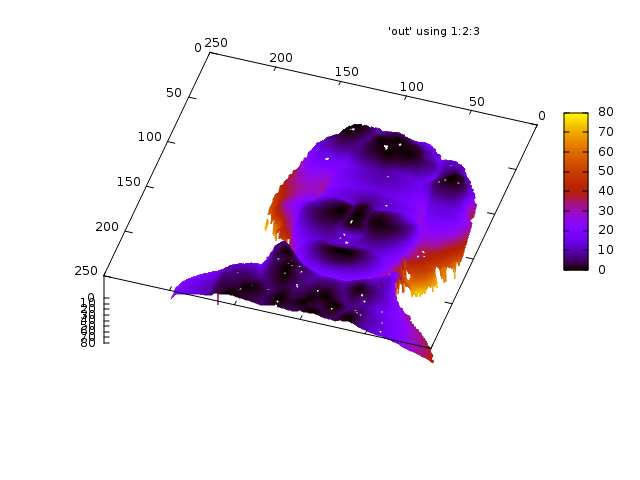
\includegraphics[width=0.5\linewidth]{img/mozart.png}
  \hfil \caption{Трехмерная поверхность Моцарта по фотографии}
  \label{fig:ex:3:out}
\end{figure}

После проверена работоспособность на фотографиях. Поскольку модель
распространения света у нас весьма упрощенная и может адекватно
обрабатывать только идеально матовые поверхности здесь результат
несколько менее точен: рисунки~\ref{fig:ex:4:in}, ~\ref{fig:ex:4:out1}
и~\ref{fig:ex:4:out2})

\begin{figure}[H]
  \centering
  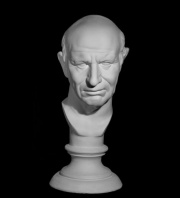
\includegraphics[width=0.5\linewidth]{img/man_in.jpg}
  \hfil \caption{исходная фотография}
  \label{fig:ex:4:in}
\end{figure}

\begin{figure}[H]
  \centering
  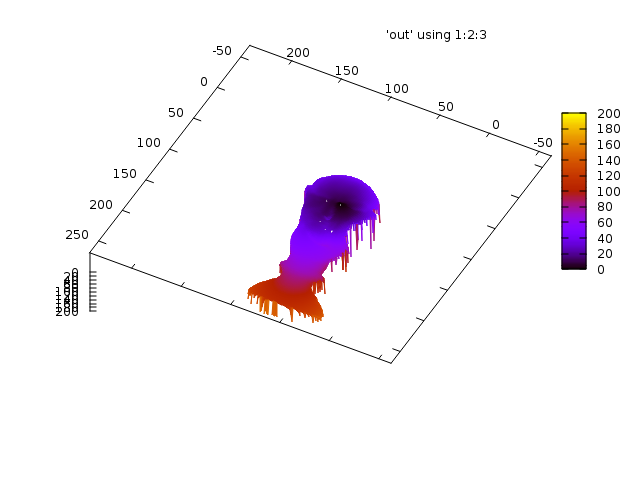
\includegraphics[width=0.5\linewidth]{img/man_all.png}
  \hfil \caption{Трехмерная поверхность по фотографии общая}
  \label{fig:ex:4:out1}
\end{figure}

\begin{figure}[H]
  \centering
  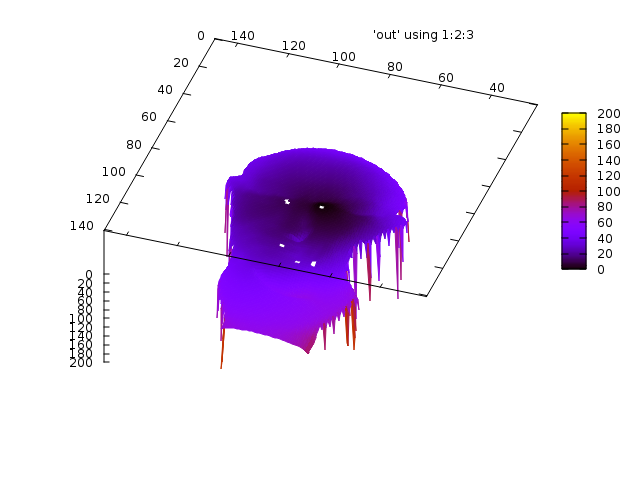
\includegraphics[width=0.5\linewidth]{img/man_detail.png}
  \hfil \caption{Детали трехмерной поверхности по фотографии }
  \label{fig:ex:4:out2}
\end{figure}


%%% Local Variables:
%%% mode: latex
%%% TeX-master: "eikonal_solver"
%%% End:

  \section{Программа}
\label{sec:program}

При реализации алгоритма использовался язык программирования python
вместе с библеотекой для научных и инженерных расчетов scipy.

Основу кода состовляет класс \emph{ImpulseSystem}, который хранит
функции $f(x)$ и $G(x)$, позволяя вычислять множество достижимости для
различных начальных данных и параметров времени. 

\begin{lstlisting}[language=Python,
caption={Интерфейс Impulse System}]
class ImpulseSystem(object):
    drift = None
    impulse = None

    def __init__(self, drift=None, impulse=None):
        self.drift = drift
        self.impulse = impulse
        self.x_0 = None
        self.ht = None
        self.h = None
        self.time = None
        self.value = None
        self.cost = dict()
        self.state_space = dict()
        self.grid_error = 0

    def integrate(self, x_0, ht, h, time, value):

    def impulse_jump(self, points_queue):

    def make_drift(self):

    def get_costs_at(self, i, j):

    def get_cost(self, cur_matrix, x, y):
\end{lstlisting}

Принци работы весьма прост. Мы создаем экземпляр класса
\emph{ImpulseSystem} отдавая ему в конструктор функции отвечающие за
дрейф --- \emph{drift} и импульсное воздействие ---
\emph{impulse}. Например для первого примера \ref{sec:snwd}. Созданный объект будет
выглядеть следующим образом:

\begin{lstlisting}[language=Python,
caption={Интерфейс Impulse System}]
F = None
G = lambda x: sc.matrix([[1 - x[1], 0], [0, 1 - x[0]]])
isys = ImpulseSystem(drift=F, impulse=G)
\end{lstlisting}

Для запуска процесса интегрирования мы вызываем метод
\emph{integrate}. На вход которому подаем все параметры --- точку
$x_0$, шаг по времени $h_t$, шаг по сетке $h$, время $T$ и ресурс $V$.

Общий процесс идет по принципу, что описан выше смотри
\ref{sec:wave_alg}. На каждом интервале сначала работает метод
\emph{impulse jump}, затем все полученные точки дрейфуют под действием
\emph{make drift} и так для всех интервалов.

После завершения работы программы мы получаем список точек, для
аппрокисмации множества достижимости.



%%% Local Variables:
%%% mode: latex
%%% TeX-master: "rs-ids"
%%% End:

  \section*{Заключение}
\label{sec:conclusion}

КОНЕЦ РАБОТЫ
%%% Local Variables:
%%% mode: latex
%%% TeX-master: "rs-ids"
%%% End:

  \pagebreak
\begin{thebibliography}{99}
  \addcontentsline{toc}{section}{Список литературы}

\bibitem{DS2011} { Dykhta~V.A., Samsonyuk~O.N.}  Some applications of
  Hamilton-Jacobi inequalities for classical and impulsive optimal
  control problems // European Journal of Control. Nonsmooth analysis,
  Control and Optimization. 2011. Vol.17. Pp. 55--69.

\bibitem{ZS1991} { Завалищин С.Т., Сесекин А.Н.}  {Импульсные
    процессы: модели и приложения}.  М.: Наука, 1991.

\bibitem{MR2005} { Миллер Б.М., Рубинович Е.Я.}  { Оптимизация
    динамических систем с импульсными управлениями}.  М.: Наука, 2005.

\bibitem{DS2003} { Дыхта В.А., Самсонюк О.Н.}  Оптимальное импульсное
  управление с приложениями.  М.: Физматлит, 2003.

\bibitem{SS2010} { Самсонюк~О.Н., Сесекин~А.Н.} Оценки и свойства
  интегральных воронок траекторий нелинейных импульсных систем //
  Тез. докл. II Международной школы-семинара «Нелинейный анализ и
  экстремальные задачи». Иркутск, ИДСТУ СО РАН, 28 июня -- 4 июля 2010
  г. 2010. С. 64--65.

\bibitem{BS2005} Вдовина О.И., Сесекин А.Н. Численное построение
  областей достижимости для систем с импульсными управлениями //
  Тр. Ин-та математики и механики УрО РАН.  2005. Т. 11, № 1.

\bibitem{FM2011} Т. Ф. Филиппова, О. Г. Матвийчук, Алгоритмы
  оценивания множеств достижи- мости импульсных управляемых систем с
  эллипсоидальными фазовыми ограничениями, Автомат. и телемех.,
  2011, выпуск 9, 127–141

\bibitem{G1997} Гурман В.И. Принцип расширения в задачах
  управления. 2-е изд., перераб. и доп. М.:Физматлит, 1997, 288 с.

\bibitem{M1993} Миллер Б.М. Метод разрывной замены времени в задачах
  оптимального управления импульсными и дискретно-непрерывными
  системами // Автоматика и телемеханика. 1993. № 12. С. 3--32.

\bibitem{MR1995} Motta M., Rampazzo F. Space-time trajectories of
  nonlinear systems driven by ordinary and impulsive controls //
  Differential Integral Equations. 1995. Vol. 8.  Pp. 269-288.

\bibitem{MS1999} Motta M., Sartori C. Discontinuous solutions to
  unbounded differential inclusions under state constraints.
  Applications to optimal control problems // Set-Valued
  Analysis. 1999. Vol. 7. Pp. 295-322.

\bibitem{WZ2007} Wolenski P.R., Zabic S.  A Sampling Method and
  Approximation Results for Impulsive Systems // SIAM J. Control
  Optim., 2007, Vol. 46. Pp. 983-998.

\bibitem{AVS2016} {Апанович Д. В.,Воронов В. А.,Самсонюк О. Н.},
  Построение множества достижимости двумерной импульсной управляемой
  системы с билинейной структурой// Изв. Иркутского
  гос. ун-та. Сер. Математика, 15 (2016), 3–16

\bibitem{AV2015_1} Апанович Д.В., Воронов В.А. Численная аппроксимация
  множеств достижимости нелинейных импульсных управляемых систем. //
  Теория управления и математическое моделирование: Тезисы докладов
  Всероссийской конференции с международным участием, посвященной
  памяти профессора Н. В. Азбелева и профессора Е. Л. Тонкова (Ижевск,
  Россия, 9–11 июня 2015 г.). Ижевск: Изд-во «Удмуртский университет»,
  2015. С. 24-25.

\bibitem{AV2015_2} Апанович Д.В., Воронов В.А. Численная аппроксимация
  неодносвязного множества достижимости нелинейной импульсной
  управляемой системы. //  Тезисы докладов III Российско-монгольской
  конференции молодых ученых по математическому моделированию,
  вычислительно-информационным технологиям и управлению (Иркутск
  (Россия) – Ханх (Монголия), 23 июня – 30 июня 2015 г.). – Иркутск:
  Научно-организационный отдел ИДСТУ СО РАН, 2015. С. 17.


\bibitem{DS2000} {Дыхта В. А., Самсонюк О.Н.} Оптимальное импульсное
  управление с приложениями. — М.: ФИЗМАТ ЛИТ, 2000. — 256 с. — ISBN
  5-9221-0097-1.

\bibitem{S1999} {J.A. Sethian.} Level Set Methods and Fast Marching Methods: evolving
interfaces in computational geometry, computer vision and matherial
science. — 2nd Ed. — Cambridge Univ. Press, 1999

\end{thebibliography}


%%% Local Variables:
%%% mode: latex
%%% TeX-master: "rs-ids"
%%% End:

  \chapter{Приложения}
\label{ch:appl}

Исходники 


\end{document}

%%% Local Variables:
%%% mode: latex
%%% TeX-master: "rs-ids"
%%% End:
